\documentclass{article}
\usepackage{pgfplots}
\pgfplotsset{compat=1.18}

\begin{document}

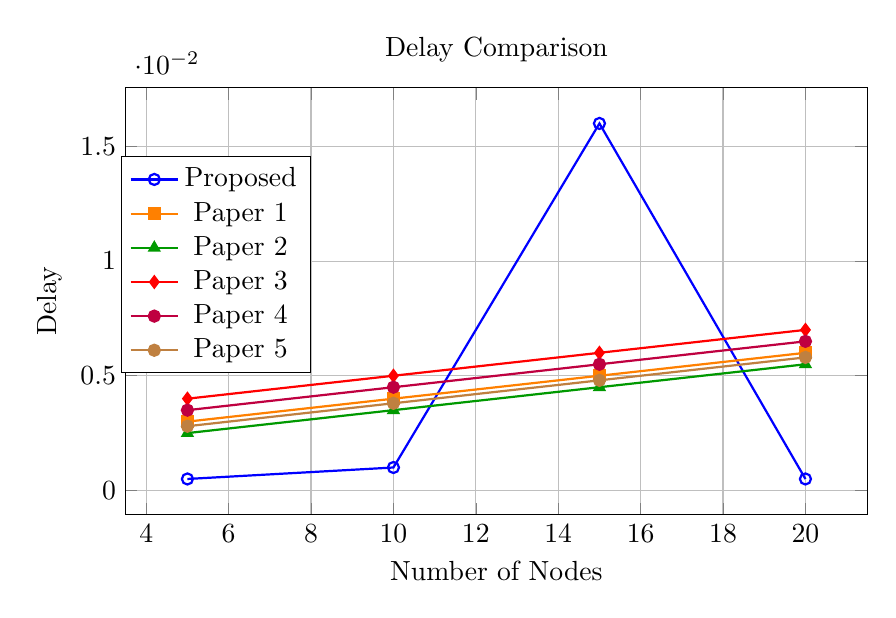
\begin{tikzpicture}
\begin{axis}[
    title={Delay Comparison},
    xlabel={Number of Nodes},
    ylabel={Delay},
    width=11cm,
    height=7cm,
    grid=major,
    legend style={
        at={(0.25,0.84)},   
        anchor=north east,
        draw=black,
        fill=white
    }
]

% Proposed (NS3)
\addplot[blue, mark=o, thick] coordinates {
    (5,0.0005) (10,0.001) (15,0.016) (20,0.0005)
};

% Paper 1
\addplot[orange, mark=square*, thick] coordinates {
    (5,0.003) (10,0.004) (15,0.005) (20,0.006)
};

% Paper 2
\addplot[green!60!black, mark=triangle*, thick] coordinates {
    (5,0.0025) (10,0.0035) (15,0.0045) (20,0.0055)
};

% Paper 3
\addplot[red, mark=diamond*, thick] coordinates {
    (5,0.004) (10,0.005) (15,0.006) (20,0.007)
};

% Paper 4
\addplot[purple, mark=*, thick] coordinates {
    (5,0.0035) (10,0.0045) (15,0.0055) (20,0.0065)
};

% Paper 5 (solid)
\addplot[brown, mark=*, thick, solid] coordinates {
    (5,0.0028) (10,0.0038) (15,0.0048) (20,0.0058)
};

\legend{Proposed, Paper 1, Paper 2, Paper 3, Paper 4, Paper 5}

\end{axis}
\end{tikzpicture}

\end{document}